\documentclass{article}
\usepackage[utf8]{inputenc}

%%%%%%%%%%%%%%%%%%%%%%%%%%%%%%%%%%%%%%%%%%%% LICENSING
% this style file is licensed under the BOOST software license 1.0
% basically, do whatever you want with this
% but please include this license information wherever you copy it

% Boost Software License - Version 1.0 - August 17th, 2003
%
% Copyright (c) 2020 Nir Elber
%
% Permission is hereby granted, free of charge, to any person or organization
% obtaining a copy of the software and accompanying documentation covered by
% this license (the "Software") to use, reproduce, display, distribute,
% execute, and transmit the Software, and to prepare derivative works of the
% Software, and to permit third-parties to whom the Software is furnished to
% do so, all subject to the following:
%
% The copyright notices in the Software and this entire statement, including
% the above license grant, this restriction and the following disclaimer,
% must be included in all copies of the Software, in whole or in part, and
% all derivative works of the Software, unless such copies or derivative
% works are solely in the form of machine-executable object code generated by
% a source language processor.
%
% THE SOFTWARE IS PROVIDED "AS IS", WITHOUT WARRANTY OF ANY KIND, EXPRESS OR
% IMPLIED, INCLUDING BUT NOT LIMITED TO THE WARRANTIES OF MERCHANTABILITY,
% FITNESS FOR A PARTICULAR PURPOSE, TITLE AND NON-INFRINGEMENT. IN NO EVENT
% SHALL THE COPYRIGHT HOLDERS OR ANYONE DISTRIBUTING THE SOFTWARE BE LIABLE
% FOR ANY DAMAGES OR OTHER LIABILITY, WHETHER IN CONTRACT, TORT OR OTHERWISE,
% ARISING FROM, OUT OF OR IN CONNECTION WITH THE SOFTWARE OR THE USE OR OTHER
% DEALINGS IN THE SOFTWARE.
%%%%%%%%%%%%%%%%%%%%%%%%%%%%%%%%%%%%%%%%%%%% /LICENSING

%%%%%%%%%%%%%%%%%%%%%%%%%%%%%%%%%%%%%%%%%%%% HOW TO USE
% some notes on using this file:
% - this file is constantly a work-in-progress; it changes frequently
% - this style file is actually split into multiple!
%   if you don't want to deal with the splitting, set the following to false
\newif\ifnirfiles
\nirfilestrue
%   otherwise, please also include sty/fitch.sty and sty/quiver.sy
%   to make the includes work, import as `\inputfrom{your/directory}{nir}`
% - this file is also split into headers that mostly commute
%   feel free to delete and move them around as you see fit
%%%%%%%%%%%%%%%%%%%%%%%%%%%%%%%%%%%%%%%%%%%% /HOW TO USE

% LTeX: enabled=false

\usepackage[margin=1in, marginparwidth=2cm]{geometry}
\usepackage[table,dvipsnames]{xcolor}
\usepackage{amsmath,amssymb,amsthm}
\usepackage{amsfonts}
\usepackage{asymptote}
\usepackage{blkarray}
\usepackage{cancel}
\usepackage{enumitem}
\usepackage{etoolbox}
\usepackage{footnotebackref}
\usepackage{graphicx}
\usepackage{mathdots}
\usepackage{mathtools} % \todo{deal with f : X -> Y to use \colon}
\usepackage{pgffor}
\usepackage{subfiles}
%\usepackage{stmaryrd}
\usepackage{textcase}
\usepackage{tikz-cd}
\usepackage{todonotes}
\usepackage{url}
\usepackage{xparse}
\usepackage{xr}

\ifnirfiles
	\usepackage{../../notes/sty/fitch}
	\usepackage{../../notes/sty/quiver}
\fi

%%%%%%%%%%%%%%%%%%%%%%%%%%%%%%%%%%%%%%%%%%%% SET-UP
\renewcommand{\familydefault}{\sfdefault}
\usepackage{cabin}
\usepackage[default]{cantarell}

\usepackage{fancyhdr}
\renewcommand{\headrulewidth}{0pt}
\fancypagestyle{contentpage}{%
	\lhead{\textit{\rightmark}}
	\cfoot{\thepage}
}

% link color stolen from wikipedia's dark blue
\definecolor{wikipediadarkblue}{rgb}{0.023, 0.270, 0.676}
\providecommand{\nirpdftitle}{notes}
\hypersetup{
	colorlinks,
	citecolor=black,
	filecolor=black,
	linkcolor=wikipediadarkblue,
	urlcolor=wikipediadarkblue,
	pdftitle={\nirpdftitle},
	pdfauthor={Nir Elber}
}
\usepackage{hyperref,cleveref}

% Labeling equations; I don't know where else to put this
\ifx\thechapter\undefined
	\numberwithin{equation}{section}
\else
	\numberwithin{equation}{chapter}
\fi
\def\equationautorefname#1#2\null{%
	(#2\null)%
}

% Bibliography
\usepackage[backend=biber,
    style=alphabetic,
    sorting=ynt
]{biblatex}
\addbibresource{../bib.bib}
\usepackage[numbib]{tocbibind}
\newcommand{\nirprintbib}{\newpage\toctrue\printbibliography[heading=bibintoc]\tocfalse}

% Table of contents
\makeatletter
\newcommand\nirtableofcontents{%
    \if@twocolumn
        \@restonecoltrue\onecolumn
    \else
        \@restonecolfalse
    \fi
    \toctrue
    \chapter*{\contentsname
        \@mkboth{%
            \MakeUppercase\contentsname}{\MakeUppercase\contentsname}} \addcontentsline{toc}{chapter}{Contents}%
    \tocfalse
    \epigraph{I encourage my fellow graduates to think about what they knew when they started out here, and how much has been layered on top of that since then. I think you'll find it's more than you had imagined.}
    {---Miles Kretschmer \cite{miles-speech}}
    \@starttoc{toc}%
    \if@restonecol\twocolumn\fi
}
\makeatother

% Sometimes I want to see the labels
\newif\ifnirdebug
\nirdebugfalse

\ifnirdebug
	\usepackage{showkeys}
\fi
%%%%%%%%%%%%%%%%%%%%%%%%%%%%%%%%%%%%%%%%%%%% /SET-UP

%%%%%%%%%%%%%%%%%%%%%%%%%%%%%%%%%%%%%%%%%%%% INDEX
\usepackage{imakeidx}
\makeindex[intoc, title=List of Definitions]
% thank you https://tex.stackexchange.com/a/299353/261927
% we are going to label each index entry with a counter
\newcounter{indexcounterlabel}
\setcounter{indexcounterlabel}{0}
\newcommand{\nirindexlabel}[1]{\label{indexentry:#1}}
\newcommand{\nirindex}[1]
{%
	\stepcounter{indexcounterlabel}%
	\nirindexlabel{\theindexcounterlabel}%
	% this command will do the labeling
	\index{#1|hyperref[indexentry:\theindexcounterlabel]}%
}
\newcommand{\nirprintindex}{\newpage\toctrue\printindex\tocfalse}
%%%%%%%%%%%%%%%%%%%%%%%%%%%%%%%%%%%%%%%%%%%% /INDEX

%%%%%%%%%%%%%%%%%%%%%%%%%%%%%%%%%%%%%%%%%%%% TITLING
\usepackage{titlesec}
\newif\iftoc

% Formatting of part
\titleformat
	{\part} % command
	[display] % shape
	{\cabin\bfseries\LARGE\scshape} % format
	{\centering\LARGE Part \thepart} % label
	{10mm} % 
	{\centering\Huge} % before-code
	[
		\thispagestyle{empty}
	] % after-code
\titlespacing*{\part}{0mm}{30mm}{30mm}
\titleclass{\part}{top}
\newcommand\partbreak{\clearpage}

% Formatting of chapter
\newif\ifinappendix% Default is \inappendixfalse
\let\oldappendix\appendix% Store \appendix
\renewcommand{\appendix}{% Update \appendix
	\oldappendix% Default \appendix
	\inappendixtrue% Set switch to true
}
\titleformat
	{\chapter} % command
	[display] % shape
	{\cabin} % format
	{} % label
	{2in} % 
	{
		% \rule{\textwidth}{1pt}
		% \vspace{1ex}
		\raggedleft
		% \\\vspace{-22pt}
		\iftoc
			\vspace{2in}
		\else%
			\ifinappendix%
				{\LARGE\textsc{Appendix}~{\thechapter}}\\
			\else%
				{\LARGE\textsc{Chapter}~{\cantarell\thechapter}}\\ % I like the other numbers ...
			\fi
		\fi
		\Huge\scshape\bfseries
	} % before-code
	[
		\vspace{-18pt}%
		\rule{\textwidth}{0.1pt}
		\vspace{0.0in}
	] % after-code
\titlespacing{\chapter}
	{0pt}
	{
		\iftoc
			-103pt+1in
		\else
			-127pt+1in
		\fi
	}
	{0pt}

% Formatting of parts
\titleformat
	{\section}
	{\Large\bfseries}
	{\thesection}
	{1em}
	{}
	[]
% varying tocdepth based on document type
\ifx\thechapter\undefined
	\setcounter{tocdepth}{1}
\else
	\setcounter{tocdepth}{2}
\fi
%%%%%%%%%%%%%%%%%%%%%%%%%%%%%%%%%%%%%%%%%%%% /TITLING

%%%%%%%%%%%%%%%%%%%%%%%%%%%%%%%%%%%%%%%%%%%% EPIGRAPH
\usepackage{epigraph}
% Thank you https://tex.stackexchange.com/a/193189
\renewcommand\textflush{flushright}

\usepackage{etoolbox}
\makeatletter
\newlength\epitextskip
\pretocmd{\@epitext}{\em}{}{}
\apptocmd{\@epitext}{\em}{}{}
\patchcmd{\epigraph}
	{\@epitext{#1}\\}
	{\vspace{-0.3in+20pt}\@epitext{#1}\\[\epitextskip]}
	{}
	{}
\makeatother

\setlength\epigraphrule{0pt}
\setlength\epitextskip{2ex}
\setlength\epigraphwidth{.6\textwidth}
\setlength\afterepigraphskip{30pt}
%%%%%%%%%%%%%%%%%%%%%%%%%%%%%%%%%%%%%%%%%%%% /EPIGRAPH

%%%%%%%%%%%%%%%%%%%%%%%%%%%%%%%%%%%%%%%%%%%% CONVENIENCE
% Various black-board things
\renewcommand{\AA}{\mathbb A}
\newcommand{\RR}{\mathbb R}
\newcommand{\ZZ}{\mathbb Z}
\newcommand{\NN}{\mathbb N}
\newcommand{\QQ}{\mathbb Q}
\newcommand{\CC}{\mathbb C}
\newcommand{\FF}{\mathbb F}
\newcommand{\OO}{\mathcal O}
\newcommand{\PP}{\mathbb P}
\newcommand{\RP}{\mathbb{RP}}
\newcommand{\CP}{\mathbb{CP}}
\newcommand{\HH}{\mathbb{H}}

\newcommand{\e}{\varepsilon}
\newcommand{\ball}[2]{(#1-#2,\,#1+#2)}

\newcommand{\floor}[1]{\left\lfloor{#1}\right\rfloor}
\newcommand{\ceil}[1]{\left\lceil{#1}\right\rceil}
\newcommand{\norm}[1]{\left\lVert{#1}\right\rVert}
\newcommand{\diff}{\operatorname{diff }}
\newcommand{\disc}{\operatorname{disc }}
\newcommand{\ord}{\operatorname{ord}}
\newcommand{\lcm}{\operatorname{lcm}}
\newcommand{\del}{\partial}
\newcommand{\emp}{\varnothing}
% \newcommand{\divides}{\,|\,}
\newcommand{\op}[1]{\operatorname{{#1}}}
\newcommand{\mf}[1]{\mathfrak{{#1}}}
\newcommand{\mc}[1]{\mathcal{{#1}}}
\newcommand{\ov}[1]{\overline{{#1}}}

\newcommand{\bb}[1]{\left\llbracket{#1}\right\rrbracket}

% Algebra
\newcommand{\coker}{\operatorname{coker}} % why isn't this a thing?!
\newcommand{\codim}{\operatorname{codim}}
\newcommand{\id}{\operatorname{id}}
\newcommand{\tr}{\operatorname{tr}}
\newcommand{\im}{\operatorname{im}}
\newcommand{\sgn}{\operatorname{sgn}}
\newcommand{\rad}{\operatorname{rad}}
\newcommand{\into}{\hookrightarrow}
\newcommand{\onto}{\twoheadrightarrow}
\newcommand{\from}{\leftarrow}
\newcommand{\eq}{\operatorname{eq}}
\newcommand{\GL}{\operatorname{GL}}

% Algebraic Geometry
\newcommand{\Spec}{\operatorname{Spec}}
\newcommand{\Proj}{\operatorname{Proj}}
\newcommand{\Pic}{\operatorname{Pic}}
\newcommand{\pre}{^{\mathrm{pre}}}
\newcommand{\sh}{^{\mathrm{sh}}}

% sheaf hom
% \makeatletter
% \DeclareFontEncoding{LS1}{}{}
% \DeclareFontSubstitution{LS1}{stix}{m}{n}
% \DeclareMathAlphabet{\mathcal}{LS1}{stixscr}{m}{n}
% \makeatother
% \DeclareMathOperator{\sHom}{\mathcal{H\mkern-7mu o\mkern-2.5mu m\mkern-1.5mu}}
% \DeclareMathOperator{\sExt}{\mathcal{E\mkern-4.5mu x\mkern-2.5mu t\mkern-1mu}}
% \DeclareMathOperator{\sEnd}{\mathcal{E\mkern-4mu n\mkern-4.5mu d\mkern-1mu}}

% Type theory
\newcommand{\refl}{\op{refl}}
\newcommand{\UU}{\mathcal{U}}

% Complex Analysis
\renewcommand{\Re}{\operatorname{Re}}
\renewcommand{\Im}{\operatorname{Im}}

% Category theory
\DeclareFontFamily{U}{dmjhira}{}
\DeclareFontShape{U}{dmjhira}{m}{n}{ <-> dmjhira }{}
\DeclareRobustCommand{\yo}{\text{\usefont{U}{dmjhira}{m}{n}\symbol{"48}}}
\newcommand{\adjoint}{\dashv}
\newcommand{\limit}{\varprojlim}
\newcommand{\colimit}{\varinjlim}
\DeclareMathOperator*{\colim}{colim}
\newcommand{\opp}{^\mathrm{op}}

% Logic
\newcommand{\lif}{\rightarrow}
\newcommand{\liff}{\leftrightarrow}
\newcommand{\bigland}{\bigwedge}
\newcommand{\biglor}{\bigvee}
\renewcommand{\models}{\vDash}
\newcommand{\nmodels}{\nvDash}
\newcommand{\dotin}{\dot{{}\in{}}}
\newcommand{\dotsubseteq}{\dot{{}\subseteq{}}}
\newcommand{\tp}{\operatorname{tp}}
\newcommand{\mapsfrom}{\mathrel{\reflectbox{\ensuremath{\mapsto}}}}

% Colons
\AtBeginDocument{%
	\mathchardef\ordinarycolon=\mathcode`:
	\mathcode`:="8000
}
\makeatletter
\newcommand{\coloncheck}{\@ifnextchar={\coloneqq\@gobble}{\ordinarycolon}}
\makeatother
\begingroup\lccode`~=`: \lowercase{\endgroup\let~}\coloncheck

\newenvironment{solution}{
\begin{proof}[Solution]}{\end{proof}}
%%%%%%%%%%%%%%%%%%%%%%%%%%%%%%%%%%%%%%%%%%%% /CONVENIENCE

%%%%%%%%%%%%%%%%%%%%%%%%%%%%%%%%%%%%%%%%%%%% DANGERS
% Thank you https://tex.stackexchange.com/a/604048
\newcommand{\nirideasymbol}{%
	
\begin{tikzpicture}[baseline=(x.base)]
		\draw[rounded corners=.01em] (-.05em,-1.07em)rectangle(.05em,.78em);
		\draw[fill=white,rounded corners=1.3] (0,.75em)--(.75em,0)--(0,-.75em)--(-.75em,0)--cycle;
		\draw[line width=0.2mm, line cap=round](-.4em,-1.07em)--(.4em,-1.07em);
		\node(x) at (0,0em) {};
		\node at (0,0em) {{\cabin\textbf{!}}};
	\end{tikzpicture}%
}
\newcommand{\nirwarnsymbol}{%
	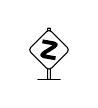
\begin{tikzpicture}[baseline=(x.base)]
		\draw[rounded corners=.01em] (-.05em,-1.07em)rectangle(.05em,.78em);
		\draw[fill=white,rounded corners=1.3] (0,.75em)--(.75em,0)--(0,-.75em)--(-.75em,0)--cycle;
		\draw[line width=0.2mm, line cap=round](-.4em,-1.07em)--(.4em,-1.07em);
		\node(x) at (0,0em) {};
		% Thank you https://tex.stackexchange.com/a/262510
		\draw[
			line cap=but,
			line join=round,
			x=.5em,
			line width=0.5mm,
			y=1*(height("Z")-\pgflinewidth)*(1-sin(10)),
			rotate=-10,
			rounded corners=1.5pt,
		](-0.57, 0.57) -- (0.57, 0.57) -- (-0.57, -0.57) -- (0.57, -0.57);
	\end{tikzpicture}%
}
%%%%%%%%%%%%%%%%%%%%%%%%%%%%%%%%%%%%%%%%%%%% /DANGERS

%%%%%%%%%%%%%%%%%%%%%%%%%%%%%%%%%%%%%%%%%%%% MARGINS
\usepackage{marginnote}
% Thank you https://tex.stackexchange.com/a/472882
% Makes marginnotes always appear on the left, apparently
%
\makeatletter
\long\def\@mn@@@marginnote[#1]#2[#3]{%
	\begingroup
		\ifmmode\mn@strut\let\@tempa\mn@vadjust\else
			\if@inlabel\leavevmode\fi
			\ifhmode\mn@strut\let\@tempa\mn@vadjust\else\let\@tempa\mn@vlap\fi
		\fi
		\@tempa{%
			\vbox to\z@{%
				\vss
				\@mn@margintest
				\if@reversemargin\if@tempswa
						\@tempswafalse
					\else
						\@tempswatrue
				\fi\fi

					\llap{%
						\vbox to\z@{\kern\marginnotevadjust\kern #3
							\vbox to\z@{%
								\hsize\marginparwidth
								\linewidth\hsize
								\kern-\parskip
								%\mn@parboxrestore
								\marginfont\raggedleftmarginnote\strut\hspace{\z@}%
								\ignorespaces#1\endgraf
								\vss
							}%
							\vss
						}%
						\if@mn@verbose
							\PackageInfo{marginnote}{xpos seems to be \@mn@currxpos}%
						\fi
						\begingroup
							\ifx\@mn@currxpos\relax\else\ifx\@mn@currpos\@empty\else
									\kern\@mn@currxpos
							\fi\fi
							\ifx\@mn@currpage\relax
								\let\@mn@currpage\@ne
							\fi
							\if@twoside\ifodd\@mn@currpage\relax
									\kern-\oddsidemargin
								\else
									\kern-\evensidemargin
								\fi
							\else
								\kern-\oddsidemargin
							\fi
							\kern-1in
						\endgroup
						\kern\marginparsep
					}%
			}%
		}%
	\endgroup
}
\makeatother
%
% Mostly for todonotes
\renewcommand{\marginpar}{\marginnote}
%%%%%%%%%%%%%%%%%%%%%%%%%%%%%%%%%%%%%%%%%%%% /MARGINS

%%%%%%%%%%%%%%%%%%%%%%%%%%%%%%%%%%%%%%%%%%%% LISTS
% Putting these into an environment decreases clicking
\newlist{listalph}{enumerate}{1}
\setlist[listalph,1]{label=(\alph*)}
\newlist{listroman}{enumerate}{1}
\setlist[listroman,1]{label=(\roman*)}
%%%%%%%%%%%%%%%%%%%%%%%%%%%%%%%%%%%%%%%%%%%% /LISTS

%%%%%%%%%%%%%%%%%%%%%%%%%%%%%%%%%%%%%%%%%%%% LISTINGS
\usepackage{courier}
\usepackage{listings}
\lstset{basicstyle=\ttfamily,breaklines=true}
%%%%%%%%%%%%%%%%%%%%%%%%%%%%%%%%%%%%%%%%%%%% /LISTINGS

%%%%%%%%%%%%%%%%%%%%%%%%%%%%%%%%%%%%%%%%%%%% THM BOXES
% See http://texdoc.net/texmf-dist/doc/latex/thmtools/thmtools.pdf
\renewcommand{\qedsymbol}{$\blacksquare$}
\usepackage{thmtools,thm-restate}

\usepackage[framemethod=TikZ]{mdframed}
% Fixing mdframed skip below
% See https://tex.stackexchange.com/a/292090/143086
\usepackage[framemethod=TikZ]{mdframed}
\usepackage{xpatch}
\makeatletter
\xpatchcmd{\endmdframed}
	{\aftergroup\endmdf@trivlist\color@endgroup}
	{\endmdf@trivlist\color@endgroup\@doendpe}
	{}{}
\makeatother

\definecolor{nirlightblue}{HTML}{f7f7ff}
\definecolor{nirdarkblue}{HTML}{1d1dbf}
\declaretheoremstyle[
	mdframed={
		backgroundcolor=nirlightblue,
		linecolor=nirdarkblue,
		rightline=false,
		topline=false,
		bottomline=false,
		linewidth=2pt,
		innertopmargin=5pt,
		innerbottommargin=8pt,
		innerleftmargin=8pt,
		leftmargin=-2pt,
		skipbelow=2pt,
		nobreak
	},
	headfont=\normalfont\bfseries\color{nirdarkblue}
]{nirbluebox}
% I want to label things by chapter, but not all things I write have chapter
\ifx\thechapter\undefined
	\declaretheorem[style=nirbluebox,name=Theorem]{thm}
\else
	\declaretheorem[style=nirbluebox,name=Theorem,within=chapter]{thm}
\fi
\declaretheorem[style=nirbluebox,name=Theorem,numbered=no]{thm*}
\declaretheorem[style=nirbluebox,name=Theorem,sibling=thm]{theorem}
\declaretheorem[style=nirbluebox,name=Theorem,numbered=no]{theorem*}
\declaretheorem[style=nirbluebox,name=Proposition,sibling=thm]{prop}
\declaretheorem[style=nirbluebox,name=Proposition,numbered=no]{prop*}
\declaretheorem[style=nirbluebox,name=Proposition,sibling=thm]{proposition}
\declaretheorem[style=nirbluebox,name=Proposition,numbered=no]{proposition*}
\declaretheorem[style=nirbluebox,name=Problem,numberwithin=section]{prob}
\declaretheorem[style=nirbluebox,name=Lemma,sibling=thm]{lem}
\declaretheorem[style=nirbluebox,name=Lemma,numbered=no]{lem*}
\declaretheorem[style=nirbluebox,name=Lemma,sibling=thm]{lemma}
\declaretheorem[style=nirbluebox,name=Lemma,numbered=no]{lemma*}
\declaretheorem[style=nirbluebox,name=Corollary,sibling=thm]{cor}
\declaretheorem[style=nirbluebox,name=Corollary,numbered=no]{cor*}
\declaretheorem[style=nirbluebox,name=Corollary,sibling=thm]{corollary}
\declaretheorem[style=nirbluebox,name=Corollary,numbered=no]{corollary*}

\definecolor{nirlightred}{RGB}{250, 220, 220}
\definecolor{nirdarkred}{HTML}{f40000}
\declaretheoremstyle[
	mdframed={
		backgroundcolor=nirlightred,
		linecolor=nirdarkred,
		rightline=false,
		topline=false,
		bottomline=false,
		linewidth=2pt,
		innertopmargin=5pt,
		innerbottommargin=8pt,
		innerleftmargin=8pt,
		leftmargin=-2pt,
		skipbelow=2pt,
		nobreak
	},
	headfont=\normalfont\bfseries\color{nirdarkred}
]{nirredbox}
\declaretheorem[style=nirredbox,name=Conjecture,sibling=thm]{conj}
\declaretheorem[style=nirredbox,name=Conjecture,numbered=no]{conj*}
\declaretheorem[style=nirredbox,name=Question,sibling=thm]{ques}
\declaretheorem[style=nirredbox,name=Question,numbered=no]{ques*}
\declaretheorem[style=nirredbox,name=Convention,sibling=thm]{conv}
\declaretheorem[style=nirredbox,name=Convention,numbered=no]{conv*}
\declaretheorem[style=nirredbox,name=Convention,sibling=thm]{convention}
\declaretheorem[style=nirredbox,name=Convention,numbered=no]{convention*}

\makeatletter
\declaretheorem[
	style=nirredbox,
	name=Idea,
	sibling=thm,
	% without \leavevmode, the first item in a list gets misformatted
	postheadhook={\leavevmode\marginnote{\nirideasymbol}[-3pt]%
	\ifthmt@thisistheone% restatable makes alignment weird
		\hspace{-2.2pt}%
	\fi}
]{idea}

\declaretheorem[
	style=nirredbox,
	name=Warning,
	sibling=thm,
	% without \leavevmode, the first item in a list gets misformatted
	postheadhook={\leavevmode\marginnote{\nirwarnsymbol}[-3pt]%
	\ifthmt@thisistheone% restatable makes alignment weird
		\hspace{-2.2pt}%
	\fi}
]{warn}
\makeatother

\definecolor{nirdarkgreen}{HTML}{20660a}
\definecolor{nirlightgreen}{HTML}{ebffeb}
\declaretheoremstyle[
	mdframed={
		backgroundcolor=nirlightgreen,
		linecolor=nirdarkgreen,
		rightline=false,
		topline=false,
		bottomline=false,
		linewidth=2pt,
		innertopmargin=5pt,
		innerbottommargin=8pt,
		innerleftmargin=8pt,
		leftmargin=-2pt,
		skipbelow=2pt,
		nobreak
	},
	headfont=\normalfont\bfseries\color{nirdarkgreen}
]{nirgreenbox}
\declaretheorem[style=nirgreenbox,name=Axiom,sibling=thm]{ax}
\declaretheorem[style=nirgreenbox,name=Axiom,numbered=no]{ax*}
\declaretheorem[style=nirgreenbox,name=Axiom,sibling=thm]{axiom}
\declaretheorem[style=nirgreenbox,name=Axiom,numbered=no]{axiom*}
\declaretheorem[style=nirgreenbox,name=Inventory,sibling=thm]{inv}
\declaretheorem[style=nirgreenbox,name=Inventory,numbered=no]{inv*}
\declaretheorem[style=nirgreenbox,name=Inventory,sibling=thm]{inventory}
\declaretheorem[style=nirgreenbox,name=Inventory,numbered=no]{inventory*}
\declaretheorem[style=nirgreenbox,name=Notation,sibling=thm]{notation}
\declaretheorem[style=nirgreenbox,name=Notation,numbered=no]{notation*}
\declaretheorem[style=nirgreenbox,name=Definition,sibling=thm]{defihelper}
\declaretheorem[style=nirgreenbox,name=Definition,numbered=no]{defihelper*}

\definecolor{nirdarkcyan}{HTML}{25805e}
\definecolor{nirlightcyan}{HTML}{edfffb}
\declaretheoremstyle[
	mdframed={
		backgroundcolor=nirlightcyan,
		linecolor=nirdarkcyan,
		rightline=false,
		topline=false,
		bottomline=false,
		linewidth=2pt,
		innertopmargin=5pt,
		innerbottommargin=8pt,
		innerleftmargin=8pt,
		leftmargin=-2pt,
		skipbelow=2pt,
		nobreak
	},
	headfont=\normalfont\bfseries\color{nirdarkcyan}
]{nircyanbox}
\declaretheorem[style=nircyanbox,name=Example,sibling=thm]{ex}
\declaretheorem[style=nircyanbox,name=Example,numbered=no]{ex*}
\declaretheorem[style=nircyanbox,name=Example,sibling=thm]{example}
\declaretheorem[style=nircyanbox,name=Example,numbered=no]{example*}
\declaretheorem[style=nircyanbox,name=Non-Example,sibling=thm]{nex}
\declaretheorem[style=nircyanbox,name=Non-Example,numbered=no]{nex*}
\declaretheorem[style=nircyanbox,name=Non-Definition,sibling=thm]{ndefi}
\declaretheorem[style=nircyanbox,name=Non-Definition,numbered=no]{ndefi*}
\declaretheorem[style=nircyanbox,name=Exercise,sibling=thm]{exercise}
\declaretheorem[style=nircyanbox,name=Exercise,numbered=no]{exercise*}
\declaretheorem[style=nircyanbox,name=Exercise,sibling=thm]{exe}
\declaretheorem[style=nircyanbox,name=Exercise,numbered=no]{exe*}

\definecolor{nirlightbrown}{RGB}{252,240,235}
\definecolor{nirdarkbrown}{HTML}{7a5342}
\declaretheoremstyle[
	mdframed={
		backgroundcolor=nirlightbrown,
		linecolor=nirdarkbrown,
		rightline=false,
		topline=false,
		bottomline=false,
		linewidth=2pt,
		innertopmargin=5pt,
		innerbottommargin=8pt,
		innerleftmargin=8pt,
		leftmargin=-2pt,
		skipbelow=2pt,
		nobreak
	},
	headfont=\normalfont\bfseries\color{nirdarkbrown}
]{nirbrownbox}
\declaretheorem[style=nirbrownbox,name=Remark,sibling=thm]{remark}
\declaretheorem[style=nirbrownbox,name=Remark,numbered=no]{remark*}
\declaretheorem[style=nirbrownbox,name=Quote,sibling=thm]{quot}
\declaretheorem[style=nirbrownbox,name=Quote,numbered=no]{quot*}
%%%%%%%%%%%%%%%%%%%%%%%%%%%%%%%%%%%%%%%%%%%% /THM BOXES

%%%%%%%%%%%%%%%%%%%%%%%%%%%%%%%%%%%%%%%%%%%% INDEX BOXES
% smuggle the note from the header formatting
\makeatletter
\def\thmt@setheadstyle#1{%
	\thmt@style@headstyle{%
		\def\NAME{\the\thm@headfont ##1}%
		\def\NUMBER{\bgroup\@upn{##2}\egroup}%
		\def\NOTE{\if=##3=\else\bgroup\thmt@space\the\thm@notefont(##3)\egroup\fi}%
		% my precious!
		\def\NIRNOTE{\if=##3=\else##3\fi}%
	}%
	\def\thmt@tmp{#1}%
	\@onelevel@sanitize\thmt@tmp
	%\tracingall
	\ifcsname thmt@headstyle@\thmt@tmp\endcsname
		\thmt@style@headstyle\@xa{%
			\the\thmt@style@headstyle
			\csname thmt@headstyle@#1\endcsname
		}%
	\else
		\thmt@style@headstyle\@xa{%
			\the\thmt@style@headstyle
			#1%
		}%
	\fi
	%\showthe\thmt@style@headstyle
}
% disable indexing in restatable, as with labels
\renewenvironment{thmt@restatable}[3][]{%
	\thmt@toks{}% will hold body
%
	\stepcounter{thmt@dummyctr}% used for data storage label.
%
	\long\def\thmrst@store##1{%
		\@xa\gdef\csname #3\endcsname{%
			\@ifstar{%
				\thmt@thisistheonefalse\csname thmt@stored@#3\endcsname
			}{%
				\thmt@thisistheonetrue\csname thmt@stored@#3\endcsname
			}%
		}%
		\@xa\long\@xa\gdef\csname thmt@stored@#3\@xa\endcsname\@xa{%
			\begingroup
			\ifthmt@thisistheone
				% these are the valid numbers, store them for the other
				% occasions.
				\thmt@rst@storecounters{#3}%
			\else
				% this one should use other numbers...
				% first, fake the theorem number.
				\@xa\protected@edef\csname the#2\endcsname{%
					\thmt@trivialref{thmt@@#3}{??}}%
				% if the number wasn't there, have a "re-run to get labels right"
				% warning.
				\ifcsname r@thmt@@#3\endcsname\else
					\G@refundefinedtrue
				\fi
				% prevent stepcountering the theorem number,
				% but still, have some number for hyperref, just in case.
				\@xa\let\csname c@#2\endcsname=\c@thmt@dummyctr
				\@xa\let\csname theH#2\endcsname=\theHthmt@dummyctr
				% disable labeling.
				\let\label=\thmt@gobble@label
				% disable indexing!
				\let\index=\@gobble
				\let\ltx@label=\@gobble% amsmath needs this
				% We shall need to restore the counters at the end
				% of the environment, so we get
				% (4.2) [(3.1 from restate)] (4.3)
				\def\thmt@restorecounters{}%
				\@for\thmt@ctr:=\thmt@innercounters\do{%
					\protected@edef\thmt@restorecounters{%
						\thmt@restorecounters
						\protect\setcounter{\thmt@ctr}{\arabic{\thmt@ctr}}%
					}%
				}%
				% pull the new semi-static definition of \theequation et al.
				% from the aux file.
				\thmt@trivialref{thmt@@#3@data}{}%
			\fi
			% call the proper begin-env code, possibly with optional argument      
			% (omit if stored via key-val)
			\ifthmt@restatethis
				\thmt@restatethisfalse
			\else
				\csname #2\@xa\endcsname\ifx\@nx#1\@nx\else[{#1}]\fi
			\fi
			\ifthmt@thisistheone
				% store a label so we can pick up the number later.
				\label{thmt@@#3}%
			\fi
			% this will be the collected body.
			##1%
			\csname end#2\endcsname
			% if we faked the counter values, restore originals now.
			\ifthmt@thisistheone\else\thmt@restorecounters\fi
			\endgroup
		}% thmt@stored@#3
		% in either case, now call the just-created macro,
		\csname #3\@xa\endcsname\ifthmt@thisistheone\else*\fi
		% and artificially close the current environment.
		\@xa\end\@xa{\@currenvir}
	}% thm@rst@store
	\thmt@collect@body\thmrst@store
}{%
	%% now empty, just used as a marker.
}
\makeatother
\declaretheoremstyle[
	mdframed={
		backgroundcolor=nirlightgreen,
		linecolor=nirdarkgreen,
		rightline=false,
		topline=false,
		bottomline=false,
		linewidth=2pt,
		innertopmargin=5pt,
		innerbottommargin=8pt,
		innerleftmargin=8pt,
		leftmargin=-2pt,
		skipbelow=2pt,
		nobreak
	},
	headfont=\normalfont\bfseries\color{nirdarkgreen},
	headformat={\NAME\ \NUMBER\NOTE{\nirindex{\NIRNOTE}}}
]{nirgreenboxindexed}
\declaretheorem[style=nirgreenboxindexed,name=Definition,sibling=thm]{defi}
\declaretheorem[style=nirgreenboxindexed,name=Definition,numbered=no]{defi*}
\declaretheorem[style=nirgreenboxindexed,name=Definition,sibling=thm]{definition}
\declaretheorem[style=nirgreenboxindexed,name=Definition,numbered=no]{definition*}
%%%%%%%%%%%%%%%%%%%%%%%%%%%%%%%%%%%%%%%%%%%% /INDEX BOXES

\pagestyle{contentpage}

\title{A More Reduced Inventory}
\author{Nir Elber}
\date{\today}
\rhead{\textit{A MORE REDUCED INVENTORY}}

\setcounter{section}{-1}

\begin{document}

\maketitle

\begin{abstract}
	We show that the classical reduced inventory for $\ZZ$ is equivalent to the statement that $\ZZ$ is initial in $\mathrm{Ring}.$
\end{abstract}

\toctrue
\tableofcontents
\tocfalse

\newpage

\section{Review of the Reduced Inventory}
In the discussion that follows, all rings have identity, as God intended. We will not require that all rings be commutative.

To review, in first-year number theory, one builds the following reduced inventory which suffices to characterize $\ZZ.$
\begin{inv}[Reduced inventory, I] \label{inv:redinvent}
	We have that $\ZZ$ is a commutative ring with the following properties.
	\begin{enumerate}
		\item There is a nonempty subset $\NN\subseteq\ZZ$ with the following properties.
		\begin{itemize}
			\item Closure: the set $\NN$ is closed under the operations $+$ and $\times.$
			\item Trichotomy: for each integer $n\in\ZZ,$ exactly one of the statements $\{-n\in\NN,n=0,n\in\NN\}$ is true. Equivalently, $\ZZ=-\NN\sqcup\{0\}\sqcup\NN.$
		\end{itemize}
		\item Well-ordering: each nonempty subset $S\subseteq\NN$ has a least element.
	\end{enumerate}
\end{inv}
Observe that well-ordering requires an ordering on $\NN,$ which one usually defines by saying
\[a<b\iff b-a\in\NN\]
for $a,b\in\ZZ.$ This defines an assymetric relation roughly because $0\notin\NN$ by trichotomy; it is transitive because $\NN$ is closed under $+.$ So indeed, $<$ provides a strict total ordering of $\ZZ.$

We are interested in showing that the single following statement is sufficient in characterizing the set of integers $\ZZ.$
\begin{inv}[Reduced inventory, II] \label{inv:zinit}
	We have that $\ZZ$ is initial in the category $\mathrm{Ring}.$
\end{inv}
Formally, our goal is to show the equivalence of \autoref{inv:zinit} and \autoref{inv:redinvent}. Work done during the number theory course can show that \autoref{inv:redinvent} implies that $\ZZ$ is initial without too much work, so we will be focusing on trying to show \autoref{inv:zinit} implies \autoref{inv:redinvent}. Nevertheless, we will show that \autoref{inv:redinvent} implies \autoref{inv:zinit} in our work later anyways.
\begin{idea}
	In fact, one can use set thoery to construct a ring $\ZZ$ which satisfies \autoref{inv:redinvent}. It is not difficult to show that \autoref{inv:redinvent} implies \autoref{inv:zinit}, so (for example) $\ZZ$ is initial in $\mathrm{Ring}$. For the other direction, any ring $R$ which is initial in $\mathrm{Ring}$ will be canonically isomorphic to $\ZZ$, and we can use this isomorphism to show that $R$ satisfies \autoref{inv:redinvent}.
\end{idea}
I don't really want to write this out, but the construction is pretty standard. I have commented out the rest of the article because its need is obviated by the above argument. I do think some of it is interesting (for example, the proof that $\NN=N(\ZZ)$), but it is mostly useless.

There is perhaps room for the possibility of a more category-theoretic argument that \autoref{inv:zinit} implies \autoref{inv:redinvent}, but I am not sure what this would look like, given that \autoref{inv:redinvent} is mostly about subsets.

% Before continuing, we issue the following warning.
% \begin{warn}
% 	Many of the proofs in this article were made quite rigorous because one must be careful in foundations. As such, the reader is encouraged to merely read the statements of results and only read the proofs which interest the reader.
% \end{warn}

% \section{Constructing Naturals}
% Anyways, we see that the main feature of $\ZZ$ according to \autoref{inv:redinvent} is that it has a very special subset $\NN\subseteq\ZZ,$ so to make \autoref{inv:zinit} work, we will need to construct this subset $\NN.$ Here is the idea.
% \begin{idea} \label{idea:natural}
% 	The subset $\NN\subseteq\ZZ$ is the subset of $\ZZ$ generated by $1$ under addition (as a monoid).
% \end{idea}
% Formalizing this requires some care. We take a moment to note that there is no reason to restrict ourselves to $\ZZ$ for the moment, for the above idea ought to apply to general rings.
% \begin{lemma} \label{lem:justifynr}
% 	Fix a ring $R.$ Then the collection
% 	\[\mathcal S(R):=\{S\subseteq R:1\in S\quad\text{and}\quad a\in S\implies a+1\in S\}\]
% 	has a unique minimum set, orderded by inclusion.
% \end{lemma}
% \begin{proof}
% 	The main point is that $\mathcal S(R)$ is closed under intersection. Namely, we simply define
% 	\[N:=\bigcap_{S\in\mathcal S(R)}S.\]
% 	Note that $1\in N$ because $1\in S$ for each $S\in S(R).$ Additionally, $a\in N$ implies that $a\in S$ for each $S\in\mathcal S(R)$ implies that $a+1\in S$ for each $S\in\mathcal S(R)$ implies that $a+1\in N.$ So indeed, the intersection $N\in\mathcal S(R).$ 
	
% 	Now, to show that $N$ is a minimum of $\mathcal S(R),$ we note that any $S\in\mathcal S(R)$ has $N\subseteq S$ by construction. The uniqueness of $N$ as a minimum element is simply because $\subseteq$ defines a partial order. So we are done.
% \end{proof}
% The above lemma justifies the following definition.
% \begin{definition}[\texorpdfstring{$N(R)$}{N(R)}]
% 	Fix a ring $R.$ Then we define the set $N(R)\subseteq R$ as the minimum of the collection
% 	\[\{S\subseteq R:1\in S\quad\text{and}\quad a\in S\implies a+1\in S\}.\]
% \end{definition}
% For the purposes of our examples, we will ignore the fact we have not defined the objects in the examples.
% \begin{example}
% 	We have that $N(\CC)=\NN.$
% \end{example}
% \begin{example}
% 	We have that $N(\ZZ/6\ZZ)=\ZZ/6\ZZ.$ Importantly, it is possible for $0\in N(\ZZ/6\ZZ).$
% \end{example}
% This condition on $N(R)$ might feel awkward, but it can be essentially rephrased as induction.
% \begin{corollary}[Induction]
% 	Fix a ring $R.$ Then the set $N(R)$ satisfies
% 	\[(S\subseteq R\quad\text{and}\quad1\in S\quad\text{and}\quad a\in S\implies a+1\in S)\implies N(R)\subseteq S.\]
% \end{corollary}
% \begin{proof}
% 	The condition on $S$ given above is simply asserting that $S\in \mathcal S(R),$ as defined in \autoref{lem:justifynr}. So $N(R)\subseteq S$ follows because $N(R)$ is the minimum of $\mathcal S(R).$
% \end{proof}
% While we're here, we pick up some facts about $N(R).$
% \begin{proposition} \label{prop:natclosed}
% 	Fix $R$ a ring. Then $N(R)$ is closed under the operations $+$ and $\times$ of $R.$
% \end{proposition}
% \begin{proof}
% 	We take the operations one at a time.
% 	\begin{itemize}
% 		\item We show that $N(R)$ is closed under addition. This means we want to show that, for any $a,b\in N(R),$ we have $a+b\in N(R).$ Equivalently, we show that $N(R)$ is a subset of
% 		\[S_+:=\{b\in R:a+b\in N(R)\text{ for each }a\in N(R)\}.\]
% 		We apply induction. Observe that $a\in N(R)$ implies that $a+1\in N(R),$ so $1\in S_+.$ Additionally, $b\in S_+$ and $a\in N(R)$ implies that $a+b\in N(R),$ so $(a+b)+1\in N(R),$ so $a+(b+1)\in N(R).$ Thus, $b+1\in S_+$ follows.
% 		\item We show that $N(R)$ is closed under multiplication. This means we want to show that, for any $a,b\in N(R),$ we have $ab\in N(R).$ Equivalently, we show that $N(R)$ is a subset of
% 		\[S_\times:=\{b\in R:ab\in N(R)\text{ for each }a\in N(R)\}.\]
% 		We apply induction. Observe that $a\in N(R)$ implies that $a\cdot1=a\in N(R),$ so $1\in S_\times.$ Additionally, $b\in S_+$ and $a\in N(R)$ implies that $ab\in N(R),$ so $ab+a\in N(R),$ so $a(b+1)\in N(R).$ Thus, $b+1\in S_\times$ follows.
% 		\qedhere
% 	\end{itemize}
% \end{proof}
% \begin{proposition} \label{prop:multcomm}
% 	Fix $R$ a ring. Then multiplication commutes in $N(R)$.
% \end{proposition}
% \begin{proof}
% 	This is another induction. Fixing some $a\in N(R)$, we have to show that $ab=ba$ for each $b\in N(R)$. (In fact, we will be able to take $a\in R$, but we will not need this generality.) So we set
% 	\[C(a):=\{b\in R:ab=ba\}.\]
% 	Observe that $1\in C(a)$ because $a\cdot1=a=1\cdot a$. Additionally, if $b\in C(a)$, then
% 	\[a(b+1)=ab+a=ba+a=(b+1)a,\]
% 	so $b+1\in C(a)$ as well. This completes the induction.
% \end{proof}
% At this point, we may say that $N(R)$ is more or less the minimal subset of $R$ which contains $1$ and is closed under addition. Namely, the definition asserts minimality under $+1,$ but this implies closure under addition as shown above anyways.

% However, \autoref{idea:natural} asserted that $N(R)$ should be generated by $1.$ While our work provides one interpretation of this, viewing ``generated'' as a minimality condition, another way to view ``generated'' is to say that every element should be a sum of $1$s. Here is a formalization of this idea.
% \begin{proposition} \label{prop:natind}
% 	Fix a ring $R.$ Then any $n\in N(R)$ has at least one of the following true.
% 	\begin{itemize}
% 		\item We have $n=1.$
% 		\item There exists $m\in N(R)$ such that $n=m+1.$ Equivalently, $n-1\in N(R).$
% 	\end{itemize}
% \end{proposition}
% \begin{proof}
% 	We proceed by contraposition: suppose that $x\in R$ has $x\ne1$ and $x-1\notin N(R).$ Then we show that $x\notin N(R).$

% 	For this, we show that $N(R)\subseteq N(R)\setminus\{x\},$ from which $x\notin N(R)$ will follow. We show this by induction.
% 	\begin{itemize}
% 		\item Observe that $1\in N(R)$ and $x\ne1$ implies that $1\in N(R)\setminus\{x\}.$
% 		\item Additionally, $a\in N(R)$ implies that $a+1\in N(R)$ as well as $a\ne x-1,$ so $a+1\ne x,$ so in fact, $a+1\in N(R)\setminus\{x\}.$
% 		\qedhere
% 	\end{itemize}
% \end{proof}
% \begin{remark}
% 	The above proposition does not assert that the two conditions are mutually exclusive. For example, $R=\ZZ/2\ZZ$ has $N(R)=R,$ in which case $1$ does have $1=0+1,$ where $0\in N(R).$
% \end{remark}
% To close out this section, we note that we acn verify our construction of the naturals is the ``correct'' one in the sense of \autoref{inv:redinvent}.
% \begin{proposition} \label{prop:natcorrect}
% 	Suppose that $\ZZ$ satisfies \autoref{inv:redinvent}. Then $N(\ZZ)=\NN.$
% \end{proposition}
% \begin{proof}
% 	We proceed by double-inclusion. As some warning, we will have to do some number theory with \autoref{inv:redinvent} during this proof.
% 	\begin{itemize}
% 		\item We show that $N(\ZZ)\subseteq\NN$ by induciton.

% 		Showing that $1\in\NN$ is somewhat subtle. By trichotomy, we have three cases.
% 		\begin{itemize}
% 			\item If $1\in\NN,$ we are done.
% 			\item If $1=0,$ then $\ZZ=\{0\}$ is the zero ring, so $\NN,$ being nonempty, must have $\NN=\ZZ,$ so $1\in\NN$ still.
% 			\item Lastly, if $-1\in\NN,$ then $(-1)(-1)=1\in\NN.$
% 		\end{itemize}
% 		To finish the induction, we note that $a\in\NN$ implies $a+1\in\NN$ by closure of $\NN$ under addition.
% 		\item We show that $\NN\subseteq N(\ZZ)$ by well-ordering. Before doing anything, we show, along the lines of \autoref{prop:natind}, that $a\in\NN$ implies $a=1$ or $a-1\in\NN.$ By trichotomy, it suffices to show that $a\not<1.$
		
% 		Well, suppose for the sake of contradiction there exists counterexample $a\in\NN$ such that $a<1$; let $m$ be the smallest such. Then $m<1$ promises $n\in\NN$ such that $m+n=1.$ But then
% 		\[m^2+mn=m<1\]
% 		implies that $m^2<1$ is a smaller counterexample as well by closure of $\NN$ under multiplication. This is our contradiction.
		
% 		We now sho wthat $\NN\subseteq N(\ZZ).$ Indeed, suppose for the sake of contradiction $\NN\setminus N(\ZZ)\subseteq\NN$ is nonempty. Then well-ordering gives us a least element, which we call $a.$

% 		Surely, $a\ne1$ because $1\in N(\ZZ).$ But then we note that $a-1\in\NN$ and is not in $\NN\setminus N(\ZZ)$ because $a$ is the smallest element. So $a-1\in N(\ZZ)$. But then $a=a-1+a\in N(\ZZ)$, which is a contradiction.
% 		\qedhere
% 	\end{itemize}
% \end{proof}

% \section{Achieving Well-Ordering}
% One might expect us to prove trichotomy for our specific ring $\ZZ$ roughly about now, but this turns out to be surprisingly subtle, as we will discuss later. For now we will content ourselves with proving well-ordering from induction and trichotomy.
% \begin{definition}[Satisfies trichotomy]
% 	Fix $R$ a ring. We say that $R$ \textit{satistfies trichotomy} if and only if, for each $r\in R,$ exactly one of $\{-r\in N(R),r=0,r\in N(R)\}$ is true. Equivalently, $R=-N(R)\sqcup\{0\}\sqcup N(R).$
% \end{definition}
% Like last time, we will ignore the fact we have not defined the objects in our examples while giving the examples.
% \begin{example}
% 	The ring $\ZZ$ should satisfy trichotomy.
% \end{example}
% \begin{nex}
% 	The ring $\CC$ does not satisfy trichotomy because $i\ne0$ and $\pm i\notin\NN.$
% \end{nex}
% \begin{nex}
% 	The ring $\ZZ/6\ZZ$ does not satisfy trichotomy because $0\in N(\ZZ/6\ZZ)=\ZZ/6\ZZ.$
% \end{nex}
% In fact, it turns out we expect $\ZZ$ to be the only ring (up to canonical isomorphism) which satisfies trichotomy because trichtomy will imply well-ordering, which then completes \autoref{inv:redinvent}.

% As discussed before, well-ordering requires an ordering. It turns out trichotomy is just a fancy way to define our ordering.
% \begin{lemma} \label{lem:ordring}
% 	Fix $R$ a ring. Define the relation $<$ by $a<b$ if and only if $b-a\in N(R).$ The relation $<$ is a strict total order on $R$ if and only if $R$ satisfies trichotomy.
% \end{lemma}
% \begin{proof}
% 	We show the directions one at a time.
% 	\begin{itemize}
% 		\item Suppose that $R$ satisfies trichotomy, and we show that $<$ is a total order.
% 		\begin{itemize}
% 			\item Irreflexive: note that $a-a=0\notin N(R)$ by trichotomy, so $a\not<a.$
% 			\item Transitive: note that $a<b$ and $b<c$ implies $b-a\in N(R)$ and $c-b\in N(R),$ so adding gives $c-a\in N(R),$ so $a<c.$
% 			\item Connected: fix $a\ne b$ so that $b-a\ne0.$ Then $b-a\in N(R)$ or $b-a\in-N(R).$ The former gives $a<b,$ and the latter gives $b<a.$
% 		\end{itemize}
% 		\item Suppose that $<$ is a total order, and we show that $R$ has trichotomy. Fix $r\in R.$ Note that $r=0$ implies that $0\not<r$ and $r\not<0.$ Additionally, $r<0$ cannot have $r=0$ or $0<r$ because $0\not<0$; similarly, $0<r$ cannot have $r=0$ or $r<0.$

% 		Thus, the conditions $\{r<0,r=0,0<r\}$ are mutually exclusive. Only now that we note $r<0$ is equivalent to $-r\in N(R),$ and $0<r$ is equivalent to $r\in N(R).$ So we indeed have trichotomy.
% 		\qedhere
% 	\end{itemize}
% \end{proof}
% And now we prove well-ordering.
% \begin{proposition} \label{lem:provewellorder}
% 	Fix $R$ a ring satisfying trichotomy. Then any nonempty subset $S\subseteq N(R)$ has a minimal element, using the ordering of \autoref{lem:ordring}.
% \end{proposition}
% \begin{proof}
% 	We start by using induction to show the result for subsets $S$ which are strictly upper-bounded. Formally, define
% 	\[T:=\{n\in N(R):\text{each nonempty }S\subseteq N(R)\text{ strictly upper-bounded by }n\text{ has a minimal}\}.\]
% 	We show that $N(R)\subseteq T$ by induction.
% 	\begin{itemize}
% 		\item Any $m\in N(R)$ has $m=1$ or $m-1\in N(R)$ by \autoref{prop:natind}, so $m=1$ or $1<m.$ In particular, $m\not<1$ is forced, so there is no nonempty subset $S\subseteq N(R)$ which is strictly upper-bounded by $1.$ So $1\in T$ vacuously.
% 		\item Suppose that $a\in T,$ and we show that $a+1\in T.$ Well, pick up any nonempty subset $S\subseteq N(R)$ which is strictly upper-bounded by $a+1.$ We have two cases.
% 		\begin{itemize}
% 			\item If $S=\{a\},$ then $a$ is a minimal element for $S.$
% 			\item Otherwise $S\setminus\{a\}$ is a nonempty subset of $N(R).$ We would like to show that $S\setminus\{a\}$ is upper-bounded by $a,$ which will give it a minimal element $m\in S\setminus\{a\}$ by induction, which will also be a minimal element for $S$ because adding in the large element $a$ doesn't matter.

% 			So pick up some $b\in S\setminus\{a\}.$ We know $b\ne a$ and $b<a+1.$ From this we get $a-b+1\in N(R)$ while $a-b\ne0$ so that $a-b+1\ne1,$ so it follows $a-b\in N(R)$ by \autoref{prop:natind} So indeed $b<a.$
% 		\end{itemize}
% 	\end{itemize}
% 	To finish, pick up a generic nonempty subset $S\subseteq N(R).$ Now, pick any $n\in S$ and define
% 	\[S':=\{s\in S:s=n\text{ or }s<n\}.\]
% 	Now, $S'\subseteq N(R)$ has a strict upper bound (e.g., $n+1$) and is nonempty because $n\in S'$, so by the discussion above, $S'$ has a minimal element. Beacuse $S$ will only add larger elements to $S',$ we see that $S$ and $S'$ share a minimal element, so $S$ has a minimal element. This finishes.
% \end{proof}
% Thus, having more or less verified well-ordering, we have reduced checking that \autoref{inv:zinit} implies \autoref{inv:redinvent} to merely showing that our initial ring $\ZZ$ satisfies trichotomy. We can codify this thinking into the following result.
% \begin{proposition} \label{prop:inv1istrich}
% 	Fix $\ZZ$ a ring. Then $\ZZ$ satisfies \autoref{inv:redinvent} if and only if $\ZZ$ satisfies trichotomy.
% \end{proposition}
% \begin{proof}
% 	If $\ZZ$ satisfies \autoref{inv:redinvent}, then \autoref{prop:natcorrect} implies that the promised subset $\NN$ is $N(\ZZ)$. Then the trichotomy of \autoref{inv:redinvent} becomes the needed trichotomy for $R$ to satisfy trichotomy.

% 	In the other direction, suppose that $\ZZ$ satisfies trichotomy. Then, setting $\NN:=N(\ZZ)$, we can check through the conditions of \autoref{inv:redinvent} to see that a ring $\ZZ$ satisfying trichotomy will satisfy each condition of \autoref{inv:redinvent}.
% 	\begin{itemize}
% 		\item Technically we must check that $\ZZ$ is a commutative ring. Fixing some $a,b\in\ZZ$, we have the following checks, by trichotomy.
% 		\begin{itemize}
% 			\item If $a=0$ or $b=0$, then $ab=ba=0$.
% 			\item If $a,b\in N(R)$, then $ab=ba$ by \autoref{prop:multcomm}.
% 			\item If $a,b\in-N(R)$, then $ab=(-a)(-b)=(-b)(-a)=ab$ by \autoref{prop:multcomm} again.
% 			\item If one of $\{a,b\}$ is in $N(R)$ while the other is in $-N(R)$, then without loss of generality, $a\in N(R)$ while $b\in-N(R)$. Then $ab=-a(-b)=-(-b)a=ba$ by \autoref{prop:multcomm} once more.
% 		\end{itemize}
% 		\item We see $\NN$ is closed under $+$ and $\times$ by \autoref{prop:natclosed}.
% 		\item We see that $\ZZ$ has the needed trichotomy directly from satisfying trichotomy.
% 		\item We see $\NN$ satisfies well-ordering by \autoref{lem:provewellorder}.
% 		\qedhere
% 	\end{itemize}
% \end{proof}

% \section{Constructing Integers}
% Trichotomy turns out to be somewhat subtle. To begin our discussion, we will get a handle on things by creating an object with weaker trichotomy.
% \begin{definition}[\texorpdfstring{$Z(R)$}{Z(R)}]
% 	Fix $R$ a ring. Then we define $Z(R):=-N(R)\cup\{0\}\cup N(R).$ Observe that we are not requiring these sets to be disjoint.
% \end{definition}
% \begin{example}
% 	We have that $Z(\CC)=\ZZ.$
% \end{example}
% \begin{example}
% 	We have that $Z(\ZZ/6\ZZ)=\ZZ/6\ZZ.$
% \end{example}
% The point of introducing $Z(R)$ is to hope that we can reduce our study of trichotmoy from general rings to the more controlled $N(R)$ by way of $Z(R).$ To this end, we quickly check that $Z(R)$ is a ring.
% \begin{proposition} \label{prop:zrisring}
% 	Fix $R$ a ring. Then $Z(R)\subseteq R$ is a subring.
% \end{proposition}
% \begin{proof}
% 	This proof is boring, and there is no reason to read it, but we will write out the checks simply to show that there is nothing clever involved. Of course, $0\in Z(R)$ and $1\in N(R)\subseteq Z(R),$ so it remains to check that $Z(R)$ is closed under $+$ and $\times.$ We take these one at a time.
% 	\begin{itemize}
% 		\item We show that $Z(R)$ is closed under $\times.$ Well, fix $a,b\in Z(R),$ and we have to show that $ab\in Z(R).$ We have the following cases.
% 		\begin{itemize}
% 			\item If either $a=0$ or $b=0,$ then $ab=0\in Z(R).$
% 			\item If $a,b\in N(R),$ then $ab\in N(R).$
% 			\item If $a,b\in-N(R),$ then $ab=(-a)(-b)\in N(R).$
% 			\item If one of $\{a,b\}$ is in $N(R)$ and the other is in $-N(R),$ then without loss of generality $a\in N(R)$ and $b\in-N(R)$ so that $-(ab)=a(-b)\in N(R),$ so $ab\in-N(R).$
% 		\end{itemize}
% 		\item We show that $Z(R)$ is closed under $+.$ Well, fix $a,b\in Z(R),$ and we have to show that $a+b\in Z(R).$ We have the following cases.
% 		\begin{itemize}
% 			\item If either $a=0,$ then $a+b=b\in Z(R).$ Similar works for $b=0.$
% 			\item If $a,b\in N(R),$ then $a+b\in N(R).$
% 			\item If $a,b\in-N(R),$ then $-(a+b)=-a+-b\in N(R),$ so $a+b\in-N(R).$
% 			\item Otherwise, as before, without loss of generality take $a\in N(R)$ and $-b\in-N(R)$ so that we want $a-b\in Z(R).$ We proceed by induction on $b.$ In particular, it suffices to show that
% 			\[N(R)\stackrel?\subseteq S_+:=\{b\in N(R):a-b\in Z(R)\text{ for each }a\in N(R)\}.\]
% 			To see that $1\in S_+,$ we note that \autoref{prop:natind} means $a\in N(R)$ implies that $a=1$ (so that $a-b=0\in Z(R)$) or $a-1\in N(R)$.

% 			Then suppose that $b\in S_+$ and fix any $a\in N(R).$ We know that $a-b\in Z(R).$ If $a-b\in-N(R),$ then $a-(b+1)\in-N(R)$ still; if $a-b=0,$ then $a-(b+1)=-1\in-N(R)$ as well.
			
% 			Otherwise $a-b\in N(R),$ and the argument above tells us that $a-(b+1)=(a-b)-1\in Z(R).$ So we have verified that $b+1\in S_+,$ as needed.
% 			\qedhere
% 		\end{itemize}
% 	\end{itemize}
% \end{proof}
% \begin{remark}
% 	In fact, $Z(R)$ can be shown to be the smallest subring of $R.$ Indeed, we already know that $Z(R)$ is a subring. On the other hand, fix $R'$ a subring. Note $0\in R'.$ Additionally, we need $1\in R',$ and closure under addition forces $a\in R'$ to imply $a+1\in R',$ so $N(R)\subseteq R'.$ Lastly, closure under negation forces each $n\in N(R)$ to have $-n\in R'.$ So indeed, $Z(R)\subseteq R'.$
% \end{remark}
% In fact, given the addition on $N(R),$ there is exactly one multiplication we can supply for $Z(R)$ which satisfies the distributive law, provided that the generator of $N(R)$ is the multiplicative identity. We will not show this here, but it follows from an induction.
% \begin{remark}
% 	In fact, $Z(R)$ is also a commutative ring. The check is identical to the one we did in \autoref{prop:inv1istrich}.
% \end{remark}

% \section{Removing Trichotomy}
% Anyways, as promised trichotomy for $Z(R)$ is easier than for general rings.
% \begin{proposition} \label{prop:easyinv1}
% 	Fix $R$ a ring. Then $0\notin N(R)$ if and only if $Z(R)$ satisfies trichotomy. Thus, $0\notin N(R)$ if and only if $Z(R)$ satisfies \autoref{inv:redinvent}.
% \end{proposition}
% \begin{proof}
% 	Technically the condition that $Z(R)$ satisfies trichotomy is that $Z(R)=-N(Z(R))\sqcup\{0\}\sqcup N(Z(R)),$ which is a bit annoying to work with, so we pick up the following coherence result.
% 	\begin{lemma} \label{lem:coherence}
% 		Fix $R$ a ring. Then $N(Z(R))=N(R).$
% 	\end{lemma}
% 	\begin{proof}
% 		Note that $1_{Z(R)}=1_R\in N(R)$ and $a\in N(R)$ implies $a+1_{Z(R)}=a+1_R\in N(R),$ so $N(Z(R))\subseteq N(R)$ by induction. Similarly, $1_R=1_{Z(R)}\in N(Z(R))$ and $a\in N(Z(R))$ implies $a+1_R=a+1_{Z(R)}\in N(Z(R)),$ so $N(R)\subseteq N(Z(R)).$ This finishes.
% 	\end{proof}
% 	While we are here, we also pick up the following, for cuteness reasons. (We will not use it anywhere.)
% 	\begin{corollary}
% 		Fix $R$ a ring. Then $Z(Z(R))=Z(R).$
% 	\end{corollary}
% 	\begin{proof}
% 		We have that $Z(Z(R))=-N(Z(R))\cup\{0\}\cup N(Z(R))$ by definition, but \autoref{lem:coherence} implies that this is $Z(Z(R))=-N(R)\cup\{0\}\cup N(R)=Z(R)$.
% 	\end{proof}
% 	Thus, $Z(R)$ satisfies trichotomy if and only if $Z(R)=-N(R)\sqcup\{0\}\sqcup N(R).$ Now, in the reverse direction, we see that $Z(R)$ satisfies trichotomy implies $0\notin N(R)$ by the nature of the disjoint union.

% 	The forward direction is more interesting. Suppose that $0\notin N(R).$ Now pick up any $a\in Z(R),$ and we have to show that exactly one of $\{a\in-N(R),a=0,a\in N(R)\}$ is true. Certainly one of them is true by construction of $Z(R).$ So we have the following cases.
% 	\begin{itemize}
% 		\item If $a=0,$ then we note $0=-0\notin N(R).$
% 		\item If $a\in N(R),$ then $a\ne0.$ Additionally, $-a\in N(R)$ would imply $a+-a=0\in N(R),$ whihch is false.
% 		\item If $a\in-N(R),$ then $a\ne-0=0.$ Additionally, $a\in N(R)$ would imply that $a+-a=0\in N(R),$ which is false.
% 		\qedhere
% 	\end{itemize}
% \end{proof}
% Because a ring satisfying trichotomy should be $\ZZ$, at this point we see that $0\notin N(R)$ is our condition of interest. For example, we can show that such rings will satisfy \autoref{inv:zinit}.
% \begin{lemma} \label{lem:atmostone}
% 	Fix $R,R'$ rings. Then there is at most one ring homomorphism $Z(R)\to R'.$
% \end{lemma}
% Note that it is possible for there to be no such map: take $R=\ZZ/6\ZZ$ and $R'=\ZZ$.
% \begin{proof}
% 	Fix two ring homomorphisms $\varphi_1,\varphi_2:Z(R)\to R'.$ We want to show that $\varphi_1(a)=\varphi_2(a)$ for each $a\in Z(R).$ We have three cases.
% 	\begin{itemize}
% 		\item Note that $\varphi_1(0)=0=\varphi_2(0)$.
% 		\item We deal with the case $a\in N(R)$ by indution. Set
% 		\[S:=\{a\in R:\varphi_1(a)=\varphi_2(a)\}.\]
% 		Note $1\in S$ because $\varphi_1(1)=1=\varphi_2(1).$ Further, if $a\in S,$ then
% 		\[\varphi_1(a+1)=\varphi_1(a)+1=\varphi_2(a)+1=\varphi_2(a+1),\]
% 		so $a+1\in S$. So it follows $N(R)\subseteq S$, as needed.
% 		\item For any $a\in-N(R)$, the previous case tells us that $\varphi_1(a)=-\varphi_1(-a)=-\varphi_2(-a)=\varphi_2(a)$.
% 		\qedhere
% 	\end{itemize}
% \end{proof}
% \begin{proposition} \label{prop:trichimpliesinitial}
% 	Fix $R$ a ring. Suppose that $0\notin N(R)$. Then $Z(R)$ is initial in $\mathrm{Ring}$.
% \end{proposition}
% \begin{proof}
% 	By \autoref{lem:atmostone}, it suffices to show that, for any ring $R',$ there exists a ring homomorphism $\varphi:Z(R)\to R'$. The main idea here is that sums of $1$s should go to sums of $1$s, which uniquely describes the morphism. Doing this formally requires some technical care.
	
% 	Fix our second ring $R'$, and note that $0\notin N(R)$ implies that $Z(R)$ satisfies trichotomy by \autoref{prop:easyinv1}, so we may give $R$ the ordering described in \autoref{lem:ordring}. Given $n\in N(R)$, we define
% 	\[R_n:=\{a\in N(R):a\le n\}.\]
% 	Observe that, by \autoref{prop:natind}, each $a\in N(R)$ has $a=1$ or $a-1\in N(R)$, so in either case $a\ge1$. In particular, if $a<n+1$, then $n+1-a\in N(R)$, so $n+1-a\ge1$, so $a\le n$. It follows that
% 	\[R_{n+1}=\{a\in N(R):a<n+1\text{ or }a=n+1\}=R_n\cup\{n+1\}.\]
% 	Now, most of the construction will be done in the following lemma.
% 	\begin{lemma}
% 		Fix any $n\in N(R)$. There is exaclty one function $\varphi:R_n\to R'$ such that $\varphi(1)=1$ and $\varphi(a+1)=\varphi(a)+1$ whenever $a,a+1\in R_n$.
% 	\end{lemma}
% 	\begin{proof}
% 		We induct on $n$; we would like to show that each $n\in N(R)$ satisfies the conclusion of the lemma.
		
% 		For $n=1$, we note that $R_1=\{1\}$: now that we know $Z(R)$ satisfies \autoref{inv:redinvent}, we see from the proof of \autoref{prop:natcorrect} that each $a\in N(R)$ has $a\ge1$, so $a\in R_1$ forces $a=1$. Thus, $\varphi(1)=1$ forces our hand for $R_1$, and this preserves addition (vacuously) and multiplication because $\varphi(1)\varphi(1)=1=\varphi(1)$.

% 		Now suppose that $n\in N(R)$ satisfies the conclusion of the lemma. For $n+1$, we note that any function $\varphi:R_{n+1}\to R'$ satisfying $\varphi(a+1)=\varphi(a)+1$ with $\varphi(1)=1$ will have $\varphi|_{R_n}:R_n\to R'$ do the same, so $\varphi|_{R_n}$ is forced. But now
% 		\[\varphi(n+1)=\varphi(n)+1\]
% 		is forced by hypothesis on $\varphi$, so $\varphi$ is forced entirely. In fact, the above discussion gives a construction of $\varphi$ which satisfies $\varphi(a+1)=\varphi(a)+1$ whenever $a,a+1\in R_n$, and then we get this also when $a,a+1\in R_{n+1}$ by noting the only extra condition to check is $a+1=n+1$, which is $\varphi(n+1)=\varphi(n)+1$.
% 	\end{proof}
% 	To finish, we let $\varphi_n:R_n\to R'$ be the functions promiseed by the lemma; by the construction of the proof, we note that $\varphi_{n+1}|_{R_n}=\varphi_n$ for each $n\in N(R)$. One can also show this more directly by using the uniqueness of the lemma.
	
% 	Now, we define $\varphi:Z(R)\to R'$ by
% 	\[\varphi(x):=\begin{cases}
% 		\varphi_x(x) & x\in N(R), \\
% 		0 & x=0, \\
% 		-\varphi_{-x}(-x) & x\in-N(R).
% 	\end{cases}\]
% 	Note that these cases are in fact disjiont because $Z(R)$ satisfies trichotomy. (Here is where we crucially use that $Z(R)$ satisfies trichotomy!) We now do casework to verify that $\varphi(a+1)=\varphi(a)+1$ for each $a\in Z(R).$
% 	\begin{itemize}
% 		\item If $a\in N(R)$, then $a+1\in N(R)$ as well, so
% 		\[\varphi(a+1)=\varphi_{a+1}(a+1)=\varphi_{a+1}(a)+1.\]
% 		It remains to show that $\varphi_{a+1}(a)=\varphi_a(a)$. But we know $\varphi_{a+1}|_{R_a}=\varphi_a$, so we are done.
% 		\item If $a=0$, then $\varphi(a+1)=1=0+1=\varphi(a)+1$.
% 		\item If $a=-1$, then $\varphi(a)+1=-1+1=0=\varphi(a+1)$.
% 		\item Otherwise, $-a\in N(R)$ and $-a\ne1$. Thus, $-a-1\in N(R)$ by \autoref{prop:natind} and in particular is nonzero, so
% 		\[\varphi(a)=-\varphi_{-a}(-a)\stackrel*=-(\varphi_{-a-1}(-a-1)+1)=\varphi(a+1)-1,\]
% 		where we have used the first case in $\stackrel*=$. This finishes.
% 	\end{itemize}
% 	From here, one can show that $\varphi$ preserves $+$ and $\times$ by hand using a few inductions and more casework, which finishes. We will not be more explicit than this because these checks are somewhat painful, and they are essentially the same as the ones in \autoref{prop:zrisring}.
% \end{proof}
% \begin{remark} \label{rem:badinitial}
% 	The condition that $0\notin N(R)$ is very important here. For example, $\ZZ/4\ZZ$ is initial in the category of rings such that $1+1+1+1=0$.
% \end{remark}
% While we're here, we note that the machinery we've built is now sufficient to show that \autoref{inv:redinvent} implies \autoref{inv:zinit}.
% \begin{theorem}
% 	Suppose that a ring $\ZZ$ satisfies \autoref{inv:redinvent}. Then $\ZZ$ satisfies \autoref{inv:zinit}; i.e., $\ZZ$ is initial in $\mathrm{Ring}$.
% \end{theorem}
% \begin{proof}
% 	By \autoref{prop:natcorrect}, we have that $N(\ZZ)=\NN.$ Additionally, by trichotomy on $\ZZ$, we see that $\ZZ=-N(\ZZ)\cup\{0\}\cup N(\ZZ)=Z(\ZZ)$. Lastly, trichotomy on $\ZZ$ (again) implies that $0\notin\NN=N(\ZZ)$, so $\ZZ=Z(\ZZ)$ is initial in $\mathrm{Ring}$ by \autoref{prop:trichimpliesinitial}.
% \end{proof}

% \section{Setting Up}
% We now return to showing that \autoref{inv:zinit} implies \autoref{inv:redinvent}. We pick up the following technical result.
% \begin{proposition} \label{prop:homonnat}
% 	Fix $R,R'$ rings. For any ring homomorphism $\varphi:R\to R'$, we have that $\varphi(N(R))=N(R').$
% \end{proposition}
% \begin{proof}
% 	Intuitively, sums of ones should go to sums of ones. Formally, we show this in two parts.
% 	\begin{itemize}
% 		\item We show that $\varphi(N(R))\supseteq N(R')$ by induction. Well, note that $1=\varphi(1)\in\varphi(N(R))$. Additionally, $a'\in\varphi(N(R))$ promises $a\in N(R)$ such that $\varphi(a)=a'$. Then $a+1\in N(R)$, so
% 		\[a'+1=\varphi(a+1)\in\varphi(N(R)).\]
% 		So indeed, $N(R')\subseteq\varphi(N(R))$ by induction.
% 		\item We show that $\varphi(N(R))\subseteq N(R')$. It suffices to show that $N(R)\subseteq\varphi^{-1}(N(R'))$, which we do by induction. Well, $\varphi(1)=1\in N(R')$, so $1\in\varphi^{-1}(N(R'))$. Additionally, $a\in\varphi^{-1}(N(R'))$ implies $\varphi(a)\in N(R'),$ so
% 		\[\varphi(a+1)=\varphi(a)+1\in N(R'),\]
% 		so $a+1\in\varphi^{-1}(N(R'))$ as well. So indeed, $N(R)\subseteq\varphi^{-1}(N(R'))$ by induction.
% 		\qedhere
% 	\end{itemize}
% \end{proof}
% The main point of this result is that we can carry around the $0\in N(R)$ condition between rings. To be explicit, we have the following.
% \begin{corollary} \label{cor:carryzero}
% 	Suppose $\ZZ$ is a ring satisfying \autoref{inv:zinit}; i.e., $\ZZ$ is initial in $\mathrm{Ring}$. Then $0\in N(\ZZ)$ if and only if $0\in N(R)$ for all rings $R$.
% \end{corollary}
% \begin{proof}
% 	Fix $R$ a ring. By hypothesis on $\ZZ$, there is a ring homomorphism $\varphi:\ZZ\to R$, and by \autoref{prop:homonnat}, we see that $0=\varphi(0)\in\varphi(N(\ZZ))=N(R)$.
% \end{proof}
% This gives the following test.
% \begin{proposition} \label{prop:thetest}
% 	Suppose there exists a ring $R$ such that $0\notin N(R)$. Then any ring $\ZZ$ satisfying \autoref{inv:zinit} will also satisfy \autoref{inv:redinvent}.
% \end{proposition}
% \begin{proof}
% 	By \autoref{cor:carryzero}, we have that $0\notin N(\ZZ)$, which implies that $Z(\ZZ)$ satisfies \autoref{inv:redinvent} by \autoref{prop:easyinv1}.
	
% 	So it remains to show that $\ZZ=Z(\ZZ)$. Note that $0\notin N(\ZZ)$ impies that $Z(\ZZ)$ is intial in $\mathrm{Ring}$ by \autoref{prop:trichimpliesinitial}, so there are unique morphisms between $\ZZ$ and $Z(\ZZ),$ so these must be isomorphisms. But there is an embedding
% 	\[Z(\ZZ)\subseteq\ZZ,\]
% 	so this must be the isomorphism $Z(\ZZ)\to\ZZ$, so $Z(\ZZ)=\ZZ$ follows.
% \end{proof}
% \begin{remark}
% 	In order to meaningfully use the condition that $\ZZ$ is intial in $\mathrm{Ring}$, one is going to need access to a large supply of rings. For example, as in \autoref{rem:badinitial}, one would not be able to distinguish $\ZZ$ from $\ZZ/4\ZZ$ if the only rings we had access to satisfied $1+1+1+1=0.$ More generally, one needs to show that no fixed finite sum of $1$s yields $0$ for all rings.

% 	What is amazing about the \autoref{prop:thetest} is that it says the above is the only obstruction, and in particular one only needs access to a single ring $R$ with $0\notin N(R)$ in order to pin down $\ZZ$.
% \end{remark}

% \section{Construction of a Ring}
% By \autoref{prop:thetest}, we see that showing \autoref{inv:zinit} implies that \autoref{inv:redinvent} comes down to construcing a ring $R$ such that $0\notin N(R)$. I am not aware of any clean way to do this.\todo{}

% At a high level, the chief annoyance with constructing such a ring $R$ is that $R$ is going to have to be an infinite set; in particular, if $N(R)$ were finite, then $(Z(R),+)$ would be a finite group, so the element $1$ would have finite additive order, forcing $0\in N(R)$.

% However, it is no easy task to construct an infinite set.

\end{document}
